\newpage
\section{Appendix}

\section{Theoretical Results}
\label{appendix:theory}

\subsection{Proof of Theorem \ref{thm:DHA_value_mu}}

\begin{T1}
    Let $\mu = (\mu_i)_{1 \leq i \leq T}$ be an admissible sequence of environments. 
    Let $\sigma = (\sigma_i)_{1 \leq i \leq k}$ be the switching times such that for all $1 \leq i < k$, $\sigma_i < \sigma_{i+1}$ and for all $1 \leq j \leq T$, $\mu_{j-1} \neq \mu_{j}$ iff $j \in \sigma$. 
    Then for any sequence of composite policies $\pi = (\pi_t)_{1 \leq t \leq T}$ with $\pi_{\mu_t} \in \pi_t$,
    \begin{multline}
        \sum_{t=1}^{T} \E_{h_{<t} \sim \mu} \left[ \left( V_{\xi}^{H}(h_{<t}, \pi_t) - V_{\mu_{t}}^{H}(h_{<t}, \pi_{\mu_t}) \right)^2 \right] \\
        \leq 2 H^3 r_{\max}^2 \log \frac{1}{w(\mu)}~,
    \end{multline}
    where $w(\mu) = \prod_{j=0}^{k} w_{\tau_j}^j$. 
\end{T1}

\begin{proof}
    The proof is split into two parts. We first define some notation and properties we will need before proving the theorem.

    \noindent\textbf{Part 1: Properties}
    
    \noindent \textbf{Induced environment models and policies.}
    For an abstract MDP $(\phi, \rho)$ where $\rho: \St \times \A \to \Dist(\St \times \Reward)$, let $\Obs(h_{<t}, sa_t) = \{o_t \in \Obs : \phi(h_{<t}ao_t) = s_t\}$.We can then define $\bar{\rho}(or_t | h_{<t}, a_t) = \bar{\rho}(r_t | h_{<t}, a_t, o_t) \bar{\rho}(o_t | h_{<t}, a_t)$ such that 
    $\sum_{o_t \in \Obs(h_{<t}, sa_t)} \bar{\rho}(o_t | h_{<t}, a_t) = \rho(s_t | s_{t-1}, a_t)$ and $\bar{\rho}(r_t | h_{<t}, a_t, o_t) = \rho(r_t | s_{t-1}, a_t)$ where $\phi(h_{<t}) = s_{t-1}$ and $\phi(h_{<t}ao_t) = s_t$. 
    For example, we can define $\bar{\rho}(o_{t} | h_{<t}, a_t)$ as:
    \begin{align*}
        \bar{\rho}(o_t | h_{<t}, a_t) = \frac{1}{\abs{\Obs(h_{<t}, sa_t)}} \rho(s_t | s_{t-1}, a_t).
    \end{align*}
    Also, for a state-dependent policy $\pi: \St \to \A$ we can define the induced history-dependent policy as $\bar{\pi}(h_{<t}) = \pi(\phi(h_{<t}))$. The crucial property is that the following equivalence holds:
    \begin{multline}
        \sum_{o_t \in \Obs} \rho(or_t | h_{<t}, \bar{\pi}(h_{<t}))
        = \sum_{s_t \in \St} \rho\left(sr_t | s_{t-1}, \pi(s_{t-1})\right) \label{eqn:1}
    \end{multline}
    % Thus, acting under policy $\bar{\pi}$ in $\bar{\rho}$ is equivalent to acting under $\pi$ in $\rho$. 
    When the context is clear, we drop the superscript on $\bar{\rho}$ and $\bar{\pi}$. Also let $\rho(sr_t | h_{<t}, a_t) = \rho(sr_t | s_{t-1}, a_t)$ where $\phi(h_{<t}) = s_{t-1}$.

    Recall that the value function under $\rho$ and $\pi$ can be expressed as:
    \begin{align*}
        V^{H}_{\rho}(h_{<t}, \pi) = \sum_{sr_{t:t+H}} \left[ \sum_{j=t}^{t+H} r_j \right] \rho(sr_{t:t+H} | h_{<t}, a_{t:t+H}),
    \end{align*}
    where $a_k = \pi(s_{k-1})$ for $k = t, \ldots, t+H$. 
    Using Equation \ref{eqn:1}, we can also express the value function in terms of observation-rewards:
    \begin{align}
        V_{\rho}^{H}(h_{<t}, \pi) &= \sum_{sr_{t:t+H}} \left[ \sum_{j=t}^{t+H} r_j \right] \rho(sr_{t:t+H} | h_{<t}, a_{t:t+H}) \nonumber\\
        &= \sum_{or_{t:t+H}} \left[ \sum_{j=t}^{t+H} r_j \right] \rho(or_{t:t+H} | h_{<t}, a_{t:t+H}). \label{eqn:2}
    \end{align}
    The actions in Equation \ref{eqn:2} are well-defined under the history-dependent policy $\bar{\pi}$.
    For notational convenience, let $\rho^{\pi}(or_{t:t+H} | h_{<t}) = \rho(or_{t:t+H} | h_{<t}, a_{t:t+H})$. 
 
    We can now also express DynamicHedgeAIXI's value function. Define the mixture environment model as:
    \begin{align*}
        \xi_j^{\pi_j}(or_{t:t+H} | h_{<t}) = \sum_{i \in M_j} \frac{w_{j, i}}{\sum_{i \in M_j} w_{j, i}} \rho_i^{\pi_i}(or_{t:t+H} | h_{<t}).
    \end{align*}
    % Here the actions under each specialist $i$ are chosen by the history-dependent policy $\bar{\pi}_i$ (induced from $\pi_i$) and we indicate this with the superscript on the action sequence. 
    The subscript $j$ indicates which time step the models in the mixture are from and also which time step the weights are from.
    
    DynamicHedgeAIXI's value function $V^{H}_{\xi}$ under $\pi_t$ can be expressed using the mixture environment model as follows:
    \begin{multline*}
        V_{\xi}^{H}(h_{<t}, \pi_t) = \sum_{i \in M_t} \frac{w_{t, i}}{\sum_{i \in M_t} w_{t, i}} V_{\rho_i}^{H}(h_{<t}, \pi_i)\\
        = \sum_{i \in M_t} \frac{w_{t, i}}{\sum_{i \in M_t} w_{t, i}} \sum_{or_{t:t+H}} \left[ \sum_{j=t}^{t+H} r_j \right] \rho_i^{\pi_i}(or_{t:t+H} | h_{<t})\\
        = \sum_{or_{t:t+H}} \left[ \sum_{j=t}^{t+H} r_j \right] \sum_{i \in M_t} \frac{w_{t, i}}{\sum_{i \in M_t} w_{t, i}} \rho_i^{\pi_i}(or_{t:t+H} | h_{<t})\\
        = \sum_{or_{t:t+H}} \left[ \sum_{j=t}^{t+H} r_j \right] \xi_t^{\pi_t}(or_{t:t+H} | h_{<t}).
    \end{multline*}

    \textbf{Predictive distribution.}
    For any environment model $\rho$ (over observation-rewards), the distribution over the next observation-reward is given by:
    \begin{align*}
        \rho^{\pi}(or_t | h_{<t}) = \frac{ \rho^{\pi}(or_{1:t}) }{ \rho^{\pi}(or_{1:t-1}) }.
    \end{align*}
    This implies for $i \leq j$, $\rho^{\pi}(or_{i:j} | h_{<i}) = \frac{ \rho^{\pi}(or_{1:j}) }{ \rho^{\pi}(or_{1:i-1}) }$. 
    % \begin{align*}
    %     \rho^{\pi}(or_{i:j} | h_{<i}) = \frac{ \rho^{\pi}(or_{1:j}) }{ \rho^{\pi}(or_{1:i-1}) }.
    % \end{align*}
    % For any environment model $\rho$, the distribution over the observation-reward at time $t$ is given by:
    % \begin{align*}
    %     \rho(or_t | h_{<t}, a_t) = \frac{\rho(or_{i:t} | h_{<i}, a_{i:t})}{\rho(or_{i:t-1} | h_{<i}, a_{i:t-1})}.
    % \end{align*}
    % The mixture model $\xi_t^{\pi}$ is also an environment model. The notation is different but we define the distribution over the observation-reward at time $t$ as:
    % \begin{align*}
    %     \xi_t^{\pi}(or_t | h_{<t}) = \frac{ \xi_t^{\pi}(or_{1:t} | h_{<i}) }{ \xi_t^{\pi}(or_{1:t-1} | h_{<i}) }
    % \end{align*}
    
    
    \textbf{Mixture model and the abstention trick.}  
    We can rewrite the mixture model using the abstention trick to instead be a mixture over all models $i \in \bar{M}_T$. % We redefine an environment model $\rho$ as:
    For an environment model $\rho$, define $\hat{\rho}$ as:
    \begin{multline*}
        \hat{\rho}(or_{t:t+H} | h_{<t}, a_t) \\
        = 
            \begin{cases}
                \rho(or_{t:t+H} | h_{<t}, a_t) &\text{if $i \in M_t$}\\
                \sum_{i \in M_t} \frac{w_{t, i}}{\sum_{i \in M_t} w_{t, i}} \rho_i(or_{t:t+H} | h_{<t}, a_t) &\text{if $i \notin M_t$}
            \end{cases}
    \end{multline*}
    Recall that the weights are defined as $w_{t, i} = e^{-L_{t-1, i}}$ (since the prior weight is equal to 1) where $L_{t-1, i} = \sum_{s \leq t-1: i \in M_s} \ell_{s, i} + \sum_{s \leq t-1: i \notin M_s} \ell_{s, i}$. 
    Let $\bar{M}_T = \bigcup_{1 \leq s \leq T} M_{s}$ denote the set of all models seen over $T$ steps and let $\pi = (\pi_i)_{i \in \bar{M}_T}$.
    Using $\hat{\rho}$, the mixture model $\xi^{\pi_t}_t$ is given by:
    \begin{multline}
        \sum_{i \in M_t} \frac{w_{t, i}}{\sum_{i \in M_t} w_{t, i}} \rho_i^{\pi_i}(or_{t:t+H} | h_{<t}) \\
        = \sum_{i \in \bar{M}_T} \frac{w_{t, i}}{\sum_{i \in \bar{M}_T} w_{t, i}} \hat{\rho}_{i}^{\pi_i}(or_{t:t+H} | h_{<t}) \\
        = \sum_{i \in \bar{M}_T} \hat{w}_{j, i} \hat{\rho}_i^{\pi_i}(or_{t:t+H} | h_{<t}), \label{eqn:mix_1}
    \end{multline}
    where $\hat{w}_{j, i} = \frac{w_{j, i}}{\sum_{i \in \bar{M}_T} w_{j, i}}$. The subscript $j$ now indicates which time step the weights are from. 
    Let $\xi_j^{\pi}(or_{t:t+H} | h_{<t}) = \sum_{i \in \bar{M}_T} \hat{w}_{j, i} \hat{\rho}_i^{\pi_i}(or_{t:t+H} | h_{<t})$. 
    From Equation \ref{eqn:mix_1}, DynamicHedgeAIXI's value function can now be expressed as:
    \begin{align*}
        V_{\xi}^{H}(h_{<t}, \pi_t) &= V_{\xi}^{H}(h_{<t}, \pi)\\
        &= \sum_{or_{t:t+H}} \left[ \sum_{j=t}^{t+H} r_j \right] \xi^{\pi}_t(or_{t:t+H} | h_{<t}).
    \end{align*}

    We will compare the value error when the value function is expressed using $\hat{\rho}$. 
    \hfill \newline

    \textbf{Part 2: Bounding the error}

    To bound the error, we first split the single sum over $t$ into a double sum over each segment between switches in the sequence $\mu$. Let $\sigma_0 = 0$ and $\sigma_{k+1} = T+1$. 
    Since $\mu_m = \mu_n$ for $\sigma_i \leq m, n \leq \sigma_{i+1}-1$, let $i$ denote the model between times $\sigma_i$ and $\sigma_{i+1}-1$ and let $\bar{\mu}_i$ denote its distribution. We thus have
    \begin{multline}
        \sum_{t = 1}^{T} \E_{h_{<t} \sim \mu} \left[ \left( V_{\xi}^{H}(h_{<t}, \pi) - V_{\mu_t}^{H}(h_{<t}, \pi_{\mu_t}) \right)^2 \right] \\
        \leq 
        \sum_{i = 0}^{k} \E\left[ \sum_{t=\sigma_i}^{\sigma_{i+1}-1} \E\left[ \left( V_{\xi}^{H}(h_{<t}, \pi) - V_{i}^{H}(h_{<t}, \pi_{i}) \right)^2 \right] \right]. \label{eqn:0}
    \end{multline}
    % For notational convenience, denote $\pi_{\bar{\mu}_i} = \pi_i$ and also let $\mu^{\pi}(or_{i:j} | h_{<i}) = \mu(or_{i:j} | h_{<i}, a_{i:j})$ where $a_k = \pi(h_{<k})$ for $k = i, \ldots, j$. 
    For $i \leq j$, define the KL divergence between two distributions over an observation-reward sequence as:
    \begin{align*}
        D_{i:j}(\mu^{\pi} || \rho^{\bar{\pi}}) = \sum_{or_{i:j}} \mu^{\pi}(or_{i:j} | h_{<i}) \log \frac{\mu^{\pi}(or_{i:j} | h_{<i})}{\rho^{\bar{\pi}}(or_{i:j} | h_{<i})}.
    \end{align*}

    Using Pinsker's inequality and the chain rule for KL divergence, the squared error can be bound as follows:
    \begin{equation}
    \begin{split}
        &\left( V_{\xi}^{H}(h_{<t}, \pi) - V_{\bar{\mu}_i}^{H}(h_{<t}, \pi_i) \right)^2 \\
        &\leq \left( \sum_{or_{t:t+H}} \left[ \sum_{j=t}^{t+H} r_j \right] \left(\xi_t^{\pi} - \bar{\mu}_i^{\pi_i}\right) \right)^2 \\
        &\leq 2 H^2 r_{\max}^2 D_{t:t+H}(\bar{\mu}_i^{\pi_i} || \xi^{\pi}_t) \\
        &= 2 H^2 r_{\max}^2 \sum_{n = t}^{t+H} \E_{h_{t:n-1} \sim \bar{\mu}_i} \left[ D_{n:n}(\bar{\mu}_i || \xi^{\pi}_t) \right].  \label{eqn:3}
    \end{split}
    \end{equation}

    Using Equation \ref{eqn:3}, over a single segment we have:
    \begin{multline}
        \sum_{t=\sigma_i}^{\sigma_{i+1}-1} \E_{h_{\sigma_i:t-1} \sim \bar{\mu}_i} \left[ \left( V_{\xi}^{H}(h_{<t}, \pi) - V_{\bar{\mu}_i}^{H}(h_{<t}, \pi_i) \right)^2 \right] \\
        \leq 
        2 H^2 r_{\max}^2 \sum_{t=\sigma_i}^{\sigma_{i+1}-1} \sum_{n=t}^{t+H} \E_{h_{\sigma_i:n-1} \sim \bar{\mu}_i} \left[ D_{n:n}(\bar{\mu}_i || \xi_n^{\pi}) \right]. \label{eqn:4}
    \end{multline}

    Let $G = \sigma_{i+1}-1 + H - \sigma_i$ and for $\sigma_i \leq t \leq \sigma_i + G$, let $l = \arg\max_{\sigma_i \leq n \leq \sigma_i + G} \left[ D_{t:t}(\bar{\mu}_i || \xi_{n}^{\pi}) \right]$. 
    Note that for each $t = \sigma_i, \ldots, \sigma_i+G$, the KL divergence term $D_{t:t}(\cdot || \cdot)$ appears at most $H$ times. Thus we have
    % \begin{multline*}
    %     \sum_{t = \sigma_i}^{\sigma_{i+1}-1} \sum_{n = t}^{t+H} \E_{h_{\sigma_i:n-1} \sim \bar{\mu}_i} \left[ D_{n:n}(\bar{\mu}_i || \xi_n^{\pi}) \right] \\
    %     \leq H \sum_{t=\sigma_i}^{\sigma_{i}+G} \E_{h_{\sigma_i:t-1} \sim \bar{\mu}_i} \left[ D_{t:t}(\bar{\mu}_i || \xi_{l}^{\pi}) \right]\\
    %     = H \cdot D_{\sigma_i: \sigma_{i+G}} (\bar{\mu}_i || \xi^{\pi}_{l}).
    % \end{multline*}
    \begin{equation}
    \begin{split}
        &\sum_{t = \sigma_i}^{\sigma_{i+1}-1} \sum_{n = t}^{t+H} \E_{h_{\sigma_i:n-1} \sim \bar{\mu}_i} \left[ D_{n:n}(\bar{\mu}_i || \xi_n^{\pi}) \right] \\
        &\leq H \sum_{t=\sigma_i}^{\sigma_{i}+G} \E_{h_{\sigma_i:t-1} \sim \bar{\mu}_i} \left[ D_{t:t}(\bar{\mu}_i || \xi_{l}^{\pi}) \right]\\
        &= H \cdot D_{\sigma_i: \sigma_{i+G}} (\bar{\mu}_i || \xi^{\pi}_{l}).
    \end{split}
    \end{equation}

    
    % The factor of $H$ arises since for each $t = \sigma_i, \ldots, \sigma_i+G$, each KL divergence term $D_{t:t}$ appears at most $H$ times in the double sum. 
    Using the fact that $\bar{\mu}_i \in \bar{M}_T$, the KL divergence term can be bound as follows:
    % $\xi_{l}^{\pi}$ is a mixture model containing $\bar{\mu}_i$,
    \begin{align}
        D_{\sigma_i: \sigma_{i+G}} (\bar{\mu}_i || \xi^{\pi}_{l}) &= \E_{h_{\sigma_{i}:\sigma_{i}+G} \sim \bar{\mu}_i} \left[ \ln \frac{\bar{\mu}_i(or_{\sigma_i:\sigma_{i}+G} | h_{<\sigma_i})}{\xi^{\pi}_l(or_{\sigma_i:\sigma_{i}+G} | h_{<\sigma_i})} \right] \nonumber \\
        &\leq \E_{h_{\sigma_{i}:\sigma_{i}+G} \sim \bar{\mu}_i} \left[ \ln \frac{1}{\hat{w}_{l, i}} \right]. \label{eqn:mix_prior_bound}
        % \sum_{or_{\sigma_i:\sigma_{i}+G}} \bar{\mu}_i(or_{\sigma_i:\sigma_{i}+G} | h_{<\sigma_i}) 
    \end{align}
    % Now note that the loss updates to the weights between time $\sigma_i$ and $l$ depend upon the reward sequence $r_{\sigma_i:l}$. 
    Define $L_{\sigma_i, j}^{l} = L_{l, j} - L_{\sigma_i, j}$. 
    Let $m = \arg\min_{j \in \bar{M}_T} L_{\sigma_i, j}^{l}$. 
    Then we have:
    \begin{equation}
    \begin{split}
        &\E_{h_{\sigma_{i}:\sigma_{i}+G} \sim \bar{\mu}_i} \left[ \ln \frac{1}{\hat{w}_{l, i}} \right] \\
        &= \E_{h_{\sigma_{i}:\sigma_{i}+G} \sim \bar{\mu}_i} \left[ \ln \frac{\sum_{j \in \bar{M}_T} w_{l, j} }{w_{l, i}} \right]\\
        % &= \E_{h_{\sigma_{i}:\sigma_{i}+G} \sim \bar{\mu}_i} \left[ \ln \frac{\sum_{j \in \bar{M}_T} w_{l, j} }{w_{l, i}} \right]\\
        &= \E_{h_{\sigma_{i}:\sigma_{i}+G} \sim \bar{\mu}_i} \left[ \ln \frac{\sum_{j \in \bar{M}_T} w_{\sigma_i, j} e^{-L_{\sigma_i, j}^{l}} }{w_{\sigma_i, i} e^{-L_{\sigma_i, i}^{l}} } \right]\\
        &\leq \log \frac{1}{\hat{w}_{\sigma_i, i}} + \E_{h_{\sigma_{i}:\sigma_{i}+G} \sim \bar{\mu}_i} \left[ - L_{\sigma_i, m}^{l} + L_{\sigma_i, i}^{l}\right].
    \end{split}
    \end{equation}
    The inequality arises by upper bounding each $e^{-L_{\sigma_i,j}^{l}}$ term in the numerator with $e^{-L_{\sigma_i,m}^{l}}$. 
    
    The term $\E_{h_{\sigma_{i}:\sigma_{i}+G} \sim \bar{\mu}_i} \left[ - L_{\sigma_i, m}^{l} + L_{\sigma_i, i}^{l}\right]$ should be upper bound by 0 since model $i$ should be the model with the smallest loss in expectation. We show this formally.
    
    Recall for a model $j$, the loss at time $t$ is given by $\ell_{t, j} = - \ln \rho_j(r_t | s_{t-1}, a_t, s_t)$ and we have $\rho_j(r_t | s_{t-1}, a_t, s_t) = \rho_j(r_t | h_{<t}, a_t, o_t)$. Thus,
    \begin{align*}
        L_{\sigma_i, j}^{l} &= - \sum_{t = \sigma_i}^{l} \ell_{t, i} \\
        &= - \sum_{t = \sigma_i}^{l} \ln \rho_j(r_t | h_{<t}, a_t, o_t).
    \end{align*}
    Thus the expectation is bound as follows:
    \begin{equation}
    \begin{split}
        &\E \left[ - L_{\sigma_i, m}^{l} + L_{\sigma_i, i}^{l}\right] \\
        &= \sum_{t = \sigma_i}^{l} \E\left[ \sum_{r_t} \bar{\mu}_i^{\pi_i}(r_t | h_{<t}, a_t, o_t) \ln \frac{ \rho^{\pi_m}_{m}(r_t | h_{<t}, a_t, o_t) }{ \bar{\mu}_i^{\pi_i}(r_t | h_{<t}, a_t, o_t) } \right]\\
        &\leq 0.
    \end{split}
    \end{equation}
    The last inequality follows since term inside the square bracket is the negative KL divergence, which is bound below 0. 

    Thus, substituting terms back into Equation \ref{eqn:4}, the bound over a single segment is given by:
    \begin{equation}
    \begin{split}
        &\sum_{t=\sigma_i}^{\sigma_{i+1}-1} \E \left[ \left( V_{\xi}^{H}(h_{<t}, \pi) - V_{\bar{\mu}_i}^{H}(h_{<t}, \pi_i) \right)^2 \right] \\
        &\leq 2 H^3 r_{\max}^2 \log \frac{1}{\hat{w}_{\sigma_i, i}} \\
        &= 2 H^3 r_{\max}^2 \log \frac{1}{\hat{w}_{\tau_i}^{i}} \label{eqn:6}
    \end{split}
    \end{equation}
    % where the last equality follows by the definition of $w_{\tau_{i}}^{i}$. 
    Combining Equation \ref{eqn:6} over $k$ segments, substituting back into Equation \ref{eqn:0}, and applying the definition of $w(\mu)$ gives the final result.    
\end{proof}


\subsection{Proof of Theorem \ref{thm:DHA_value_constant}}

Theorem \ref{thm:DHA_value_constant}, restated below, follows from Theorem \ref{thm:DHA_value_mu} by bounding $w(\mu)$.

\begin{T2}
    Let $\mu = (\mu_i)_{1 \leq i \leq T}$ be an admissible sequence of environments. Let $\sigma = (\sigma_i)_{1 \leq i \leq k}$ be the switching times such that $\sigma_i < \sigma_{i+1}$ and $\mu_{i-1} \neq \mu_{i}$ only when $i = \sigma_{i}$.
    Let $\bar{M}_t = \bigcup_{0 \leq s \leq t} M_s$. 
    Then for any sequence of composite policies $\pi = (\pi_t)_{1 \leq t \leq T}$ with $\pi_{\mu_t} \in \pi_t$,
    \begin{align}
        \sum_{t=1}^{T} \E_{h_{<t} \sim \mu} \left[ \left( V_{\xi}^{H}(h_{<t}, \pi_t) - V_{\mu_{t}}^{H}(h_{<t}, \pi_{\mu_{t}}) \right)^2 \right] \nonumber\\
        \leq 4 k H^3 r_{\max}^2 \log \abs{\bar{M}_T}~.
    \end{align}
\end{T2}

\begin{proof}
    Start with the bound provided in Theorem \ref{thm:DHA_value_mu}. The term $w(\mu)$ is given by ${w(\mu) = \sum_{j=1}^{k} \log \frac{1}{\hat{w}_{\tau_j}^j}}$. The weight $w_{\tau_j}^j$ can be expressed as
    \begin{align*}
        \hat{w}_{\tau_j}^j &= \frac{ e^{-L_{\tau_j-1, j}} }{ \sum_{i \in \bar{M}_{T}} e^{-L_{\tau_j-1, i}} }\\
        &= \frac{ 1 }{ \sum_{i \in \bar{M}_{T}} e^{L_{\tau_j-1, j}-L_{\tau_j-1, i}} }
    \end{align*}

    Recall that $L_{t, i} = \sum_{s \leq t: i \in M_s} \ell_{s, i} + \sum_{s \leq t: i \notin M_s} \ell_s$. So each model incurs DynamicHedge's loss until the time they enter. Therefore only models $i \in \bar{M}_T$ with $\tau_i < \tau_j$ differ in their loss compared to model $j$. Thus for any $i \in \bar{M}_T$ such that $\tau_i < \tau_j$,
    \begin{align*}
        L_{\tau_j - 1, j} - L_{\tau_j - 1, i} &= \sum_{t = \tau_i}^{\tau_j - 1} \ell_t - \ell_{t,i}\\
        &\leq \log \abs{\bar{M}_T}~,
    \end{align*}
    where $\bar{M}_T = \bigcup_{1 \leq s \leq t} M_s$ is the set of all models seen by the agent up to time $T$. The inequality follows from Hedge's regret bound (Proposition \ref{prop:hedge_regret}) and generating a prior from the unnormalized prior weight by multiplying by $\frac{1}{\abs{\bar{M}_T}}$. Thus we have that $\hat{w}_{\tau_j}^j$ is lower bounded by
    \begin{align*}
        w_{\tau_j}^j &\geq \frac{1}{\sum_{i \in \bar{M}_T} \abs{\bar{M}_T}}\\
        &\geq \frac{1}{\abs{\bar{M}_T}^2}.
    \end{align*}
    Substituting this back into our value bound gives our final result.
\end{proof}



\section{Design of Experiments}
\label{appendix:design_of_experiments}
We describe the details of our experiment design in this section. 
All experiments were performed on a shared server with a 32-Core Intel(R) Xeon(R) Gold 5218 CPU and 192 gigabytes of RAM.


\subsection{Dynamic Knowledge Injection Setup}
We simulate the dynamic knowledge injection setting by maintaining two sets of predicates $I$ and $U$ representing the informative and uninformative predicates for each domain. Given a proportion $p \in [0, 1]$, a new $\Phi$-BCTW model of depth $d$ is constructed by sampling $\lfloor p \cdot d \rfloor$ predicates from $I$ and $d - \lfloor p \cdot d \rfloor$ predicates from $U$. The proportion $p$ initially starts out small and increases over time.

In all our experiments, we drop the $\Phi$-BCTW model with the lowest DynamicHedge weight and introduce a new $\Phi$-BCTW model every $4$K steps. The model is also pre-trained on the preceding $4$K steps to ensure it does not perform too poorly to when it is first introduced. The parameter $p$ starts out at $p = 0.05$ and increases by $0.05$ every $4$K steps. 

\iffalse
    \begin{itemize}
        \item Let $U$ and $I$ denote the set of uninformative and informative predicates.
        \item Given $p \in [0, 1]$ and the depth parameter $d$ of a $\Phi$-BCTW model, return a set of $d$ predicates where $\lfloor p \cdot d \rfloor$ are sampled from $I$ and $d - \lfloor p \cdot d \rfloor$ are sampled from $U$.
        \item Every 4k steps, we introduce a new $\Phi$-BCTW model generated using a predicate step generated this way. This model is pre-trained on the preceding 4k steps before it is sent to the agent. This ensures that it does not perform too poorly to start. 
        \item The parameter $p$ is increased by $0.05$ (until a max of 1) every time a new model is introduced. 
    \end{itemize}
\fi



\subsection{Environment Design}
We now describe the design of each environment, the parameters used, and the predicates used.
The following functions help us deal with binary representations:
\begin{itemize}
    \item $\it{Encode}_i$ splits the possible range of its argument into $2^i$ equal sized buckets and encodes its argument by the number of whichever bucket it falls into. If the range is unbounded, it is first truncated. 
    \item $\it{Bit}_i$ takes a bit string and returns the $i$th bit. 
    \item $(= 1)$ returns whether the provided argument equals 1.
    \item $(\geq p)$ returns whether the provided argument is greater than $p$.
\end{itemize}

Function composition\index{composition ($\comp$)} is handled by the (reverse)
composition function 
\[ \comp : (a \rightarrow b) \rightarrow (b \rightarrow c) \rightarrow 
             (a \rightarrow c) \]
defined by
$ ((f \comp g) \; x) = (g \; (f \; x)).$

\textbf{Biased Rock-Paper-Scissors (RPS).} 
As mentioned in Section 5.1, there are two informative predicates in this domain: $IsRock_{t-1}(h)$ and $IsLose_{t-1}(h)$ indicate whether the envionment played rock and whether the agent lost in the previous time step respectively. The $\Phi$-BCTW models introduced in this domain are all constructed to have depth 2. 

\textbf{Taxi.} 
We modify the original taxi environment of \cite{FMVRW07}, such that a 2x5 grid is used instead. The passenger and destination still spawn in the corner locations with coordinates $(0,0), (1,0), (0, 4), (1,4)$. The agent receives -1 reward for running into a wall, +100 reward for successfully dropping off the passenger at its destination. The observation received at each time step is the state $(x, y, p, d)$ where $(x, y)$ denote the position of the agent (representing the taxi), $p$ is an index indicating the passenger position, and $d$ is an index indicating the destination position. The agent has access to informative predicate functions of the following forms:
\begin{itemize}
    \item $\it{xDistToPassenger}_{1} \comp Encode_n \comp Bit_i \comp (= 1)(h)$ - $\it{xDistToPassenger}_{1}$ takes a history sequence and returns the $x$ distance from the agent to the passenger at the last time step. The predicate returns whether the $i$th bit of the $x$ distance encoded into $n$ bits equals 1. 
    \item $\it{yDistToPassenger}_{1} \comp Encode_n \comp Bit_i \comp (= 1)(h)$ - $\it{yDistToPassenger}_{1}$ takes a history sequence and returns the $y$ distance from the agent to the passenger at the last time step. The predicate returns whether the $i$th bit of the $y$ distance encoded into $n$ bits equals 1. 
    \item $\it{xDistToDestination}_{1} \comp Encode_n \comp Bit_i \comp (= 1)(h)$ - $\it{xDistToDestination}_{1}$ takes a history sequence and returns the $x$ distance from the agent to the destination at the last time step. The predicate returns whether the $i$th bit of the $x$ distance encoded into $n$ bits equals 1. 
    \item $\it{yDistToDestination}_{1} \comp Encode_n \comp Bit_i \comp (= 1)(h)$ - $\it{yDistToDestination}_{1}$ takes a history sequence and returns the $y$ distance from the agent to the destination at the last time step. The predicate returns whether the $i$th bit of the $y$ distance encoded into $n$ bits equals 1. 
    \item $\it{PassengerPickedUp}(h)$ - Takes a history sequence $h$ and returns whether the passenger was in the taxi at the last time step. 
    \item $\it{Suffix}_N \comp (= 1) (h)$ - Returns whether the $N$th bit of the suffix of the history in binary representation equals 1. The agent will recover the original MDP if it captures the indicator functions that comprise the last received observation.
\end{itemize}

The $\Phi$-BCTW models introduced in this domain are constructed from a set of $17$ predicates. 

\textbf{Epidemic Control over Contact Networks.}
We delay the full description of the epidemic control environment and the parameters used until Appendix \ref{appendix:SEIRS_dynamics} but describe the predicates used here. We assume that the agent has a background theory consisting of:
\begin{itemize}
    \item A graph $G = (V, \mathcal{E})$ that captures (approximately) the structure of the underlying contact network, but ont the disease status of nodes. The connectivity between individuals could be inferred from census data, telecommunication records, contact tracing apps etc.
    \item The transition and observation functions of a dynamics model of the underlying disease but not the parameters. This information would be provided by experts in the domain, such as epidemiologists working on epidemic modelling. 
\end{itemize}

The following functions are defined:
\begin{itemize}
    \item $\it{NaiveInfectionRate}_{t, \nu}$ takes a history sequence $h \in \Hist$ and computes the infection rate at time $t$ over `the set of nodes $\nu \subseteq V$ as the observed infection rate plus a constant multiplied by the number of nodes observed as unknown.
    \item $\it{InfectionRateOfChange}_{t, \nu}$ takes a history sequence $h \in \Hist$ and computes the change in infection rate between timesteps $t-1$ and $t$ over the set of nodes $\nu \subseteq V$. 
    \item $\it{PercentAction}_{a, N}$ takes a history and returns the percentage of time action $a$ was selected in the last $N$ timesteps.
    \item $\it{ActionSequenceIndicator}_{a_{1:k}}$ is an indicator function returning 1 if the last $k$ actions performed match $a_{1:k}$ and 0 otherwise.
    \item $\it{MAReward}_w$ takes a history and returns the moving average of the reward over a window of size $w$. 
    \item $\it{RateOfChange}$ takes two real numbers and computes the ratio between them.
    \item $\it{ParticleFilter}_{\theta, M}$ takes a history sequence and approximates the belief state using the transition and observation models given by $\theta$ and $M$ particles.
    \item $\it{ParticleInfRate}$ takes a belief state represented by a set of particles and computes the expected infection rate. 
\end{itemize}

The agent has access to the following predicate functions:
\begin{itemize}
    \item $\it{NaiveInfectionRate}_{t, \nu} \comp \it{Encode}_5  \comp \it{Bit}_i \comp (=1) (h) \;\;\; \text{for various } \;i, \nu \subseteq V, \; t = 1$
    \item $\it{InfectionRateOfChange}_{t, \nu} \comp  \it{Encode}_{7}  \comp \it{Bit}_i \comp (=1) (h) \;\;\; \text{for various} \;i, \nu \subseteq V, \; t = 1$
    \item $\it{PercentAction}_{a, N} \comp \it{Encode}_{8}  \comp \it{Bit}_i \comp (=1) (h) \;\;\; \text{for all } a \in \A  \text{ and various values of } N$
    \item $\it{ActionSequenceIndicator}_{a_{1:k}}(h)$ for various $a_{1:k}$, 
 ${k \geq 1}$
    \item $\lambda s.\it{RateOfChange}(\it{MAReward}_{w_1}(s), $ $\it{MAReward}_{w_2}(s)) \comp $ ${( \geq 1) (h)}$ \text{for } $w_1, w_2 \in \N$
    \item $\it{ParticleFilter}_{\theta, M} \comp \it{ParticleInfRate} \comp \it{Encode}_5  \comp \it{Bit}_i \comp$ ${(=1)(h)}$ for various $\theta, M = 100$
\end{itemize}

The $\Phi$-BCTW models introduced in this domain are constructed from a set of $20$ predicates. 

\textbf{Uninformative Predicates.}
The set of uninformative predicates contains predicates that provide limited utility in representing the environment. The most basic uninformative function we generate is $\it{RandomBit}_{p}$ which returns $1$ with probability $p$ and $0$ otherwise. We also consider a predicate function $\it{Randomize}_{p}$ which takes a binary symbol as input and outputs the same symbol with probability $p$. $\it{Randomize}_{p}$ is used to produce noised versions of the informative predicates; given a predicate function $f: \Hist \to \{0, 1\}$, $\it{Randomize}_{p}$ can be used to define a predicate function $f \comp \it{Randomize}_{p}(h)$. Whilst randomized versions of the informative predicates are not strictly `uninformative' (depending on the level of randomization), the level of utility they provide is typically lower than their non-randomized counterparts. 


\subsection{Agent Design}
Table \ref{tab:BCTW_config} details the agent configuration used in each domain. The $\abs{M_t}$ column denotes the maximum number of specialists that are available at any one time. 
The $d$ column denotes the number of predicates used to construct the $\Phi$-BCTW model and consequently, the depth of the $\Phi$-BCTW tree. 
The $\epsilon$ column denotes the starting value of $\epsilon$ used in $\epsilon$-greedy exploration and the decay factor column denotes the rate at which the value of $\epsilon$ decreases after each time step. 
Finally, the $H$ column denotes the horizon used to compute the value function and MCTS simulations denotes the number of MCTS simulations computed per time step.

\begin{center}
    \begin{table}[H]
        \centering
        \begin{tabular}{cccc}
         & Biased RPS & Taxi & Epidemic Control\\
        \hline
        $\abs{M_t}$ & 10 & 10 & 10\\
        $d$ & 2 & 17 & 20 \\
        $\epsilon$ & 0.999 & 0.999 & 0.9999\\
        Decay factor & 0.9999 & 0.9999 & 0.999999\\
        $H$ & 4 & 14 & 10\\
        MCTS Sims & 40 & 50 & 20
        \end{tabular}
        \caption{DynamicHedgeAIXI agent learning configuration for each domain.}
        \label{tab:BCTW_config}
    \end{table}
\end{center}


\section{SEIRS epidemic process on contact networks}
\label{appendix:SEIRS_dynamics}

\begin{figure}[H]
    \centering
    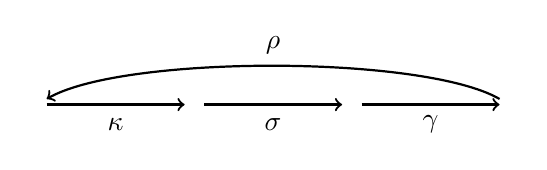
\begin{tikzpicture} %[baseline=(s1.base)]
        % SEIRS states
        \node (s2) at (6,0) {$\sS$};
        \node (e2) at (8,0) {$\sE$};
        \node (i2) at (10,0) {$\sI$};
        \node (r2) at (12,0) {$\sR$};
        % SEIRS transitions
        \draw [->,thick] (s2) to (e2) node[draw=none] at (7,-.25) {$\kappa$};
        \draw [->,thick] (e2) to (i2) node[draw=none] at (9,-.25) {$\sigma$};
        \draw [->,thick] (i2) to (r2) node[draw=none] at (11,-.25) {$\gamma$};
        \draw [->,thick,bend right] (r2) to [looseness=.5] (s2) node[draw=none] at (9, .75) {$\rho$};
    \end{tikzpicture}
    \caption{SEIRS compartmental model on contact networks with transmission rate $\kappa = \frac{1-(1-\beta)^{k_t}}{\omega}$ (where $\beta$ is the contact rate), latency rate $\sigma$, recovery rate $\gamma$ and loss of immunity rate $\rho$. }
    \label{fig:epi}
\end{figure}

We model the epidemic control problem as a stochastic Susceptible-Exposed-Infected-Recovered-Susceptible (SEIRS) process evolving over a contact network.
A contact network is an undirected graph where the nodes represent individuals and the edges represent interactions between individuals. Each individual node in the graph is labelled by one of four states corresponding to their infection status: Susceptible ($\sS$), Exposed ($\sE$), Infectious ($\sI$), and Recovered ($\sR$). Every node also maintains an immunity level $\omega$. The model evolves as a POMDP. At time $t$, the temporal graph is given by $G_t = (V, \mathcal{E}_t)$ with $V$ as the set of nodes and $\mathcal{E}_t$ as the set of edges at time $t$. A function $\zeta_t : V \to \{\sS, \sE, \sI, \sR\} \times \{1, \eta_1, \eta_2\}$ maps each node to its label and one of three immunity levels where $\eta_1, \eta_2 \in  \R_+$. Together, $(G_t, \zeta_t)$ constitute the state. 
% Figure \ref{fig:epi} depicts the dynamics of how a node transitions between states. 
At time $t$, a Susceptible node with $k_t$ Infectious neighbours becomes Exposed with probability $\frac{1-(1-\beta)^{k_t}}{\omega}$, where $\beta \in [0, 1]$ is the rate of transmission. An Exposed node becomes Infectious at rate $\sigma$. Similarly, an Infectious node becomes Recovered at a rate $\gamma$ and becomes Susceptible again at a rate $\rho$.

The agent performs an action $a_t$. Quarantine actions modify the underlying connectivity of the graph $G_t$ by removing any edges that contain a quarantined node; this leads to the graph at time $t+1$, $G_{t+1}$. Vaccinate actions modify $\zeta_{2, t}$ such that vaccinated nodes have updated immunity levels in $\zeta_{2, t+1}$. The infection status label of every node evolves according to the following equations:
\begin{equation}
\begin{split}
&\tau(\zeta_{1, {t+1}}(v) | \zeta_{1, t}(v), s_t ) \\
&= 
\begin{cases}
    \frac{1 - (1 - \beta)^{k_t}}{\zeta_{2, t}(v)} \;\; & \text{if } \zeta_{1, {t+1}}(v) = E \text{ and }\zeta_{1, t}(v) = S\\
    1 - \frac{1 - (1 - \beta)^{k_t}}{\zeta_{2, t}(v)} \;\; & \text{if } \zeta_{1, {t+1}}(v) = S \text{ and }\zeta_{1, t}(v) = S\\
    \sigma \;\; & \text{if } \zeta_{1, {t+1}}(v) = I \text{ and }\zeta_{1, t}(v) = E\\
    1 - \sigma \;\; & \text{if } \zeta_{1, {t+1}}(v) = E \text{ and }\zeta_{1, t}(v) = E\\
    \gamma \;\; & \text{if } \zeta_{1, {t+1}}(v) = R \text{ and }\zeta_{1, t}(v) = I\\
    1 - \gamma \;\; & \text{if } \zeta_{1, {t+1}}(v) = I \text{ and }\zeta_{1, t}(v) = I\\ 
    \rho \;\; & \text{if } \zeta_{1, {t+1}}(v) = S \text{ and }\zeta_{1, t}(v) = R\\
    1 - \rho \;\; & \text{otherwise,}
\end{cases}
\label{eqn:SEIRS_transition}
\end{split}
\end{equation}
where $k_t$ denotes the number of Infectious, connected neighbours that $v$ has at time $t$.

The observations resemble the testing for an infectious disease with positive $+$ and negative $-$ outcomes. Recall that the observations on each node are from $\Obs = \{+, -, ?\}$ where $?$ indicates the corresponding individual has unknown/untested status. At time $t$, node $v \in V$ emits an observation according to the following distribution:
\begin{equation}
% \label{eq:seirs:obs}
\begin{split}
    & \xi_t^{v}(+ | \zeta_{1, t}(v) = S) = \alpha_S \mu_S, \\
    & \xi_t^{v}(+ | \zeta_{1, t}(v) = E) = \alpha_E \mu_E, \\
    & \xi_t^{v}(- | \zeta_{1, t}(v) = S) = \alpha_S (1 - \mu_S), \\
    &\xi_t^{v}(- | \zeta_{1, t}(v) = E) = \alpha_\sE (1-\mu_E), \\
    & \xi_t^{v}(? | \zeta_{1, t}(v) = S) = 1 - \alpha_S, \\
    &\xi_t^{v}(? | \zeta_{1, t}(v) = E) = 1 - \alpha_E, \\
    & \xi_t^{v}(+ | \zeta_{1, t}(v) = I) = \alpha_I \mu_I, \\
    &\xi_t^{v}(+ | \zeta_{1, t}(v) = R) = \alpha_R \mu_R, \\
    & \xi_t^{v}(- | \zeta_{1, t}(v) = I) = \alpha_I (1-\mu_I), \\ 
    &\xi_t^{v}(- | \zeta_{1, t}(v) = R) = \alpha_R (1 - \mu_R), \\
    & \xi_t^{v}(? | \zeta_{1, t}(v) = I) = 1 - \alpha_I, \\
    & \xi_t^{v}(? | \zeta_{1, t}(v) = R) = 1 - \alpha_R.
\end{split}
\label{eqn:SEIRS_obs}
\end{equation}

Here, $\alpha_S, \alpha_E, \alpha_I, \alpha_R$ denote the fraction of Susceptible, Exposed, Infectious and Recovered individuals, respectively, that are tested on average at each time step. The parameters $\mu_S, \mu_E, \mu_I, \mu_R$ denote the probability that a node that is Susceptible, Exposed, Infectious, Recovered respectively tests positive.
Table \ref{tab:trans_obs_params} lists the transition and observation model parameters that were used.
% in all experiments.

\begin{center}
    \begin{table}[H]
        \begin{center}
        \begin{tabular}{cc}
        Parameter & Value\\
        \hline
        $\beta$ & 0.2\\
        $\sigma$ & 0.3\\
        $\gamma$ & 0.08\\
        $\rho$ & 0.1\\
        $\alpha_S$ & 0.1\\
        $\alpha_E$ & 0.1\\
        $\alpha_I$ & 0.8\\
        $\alpha_R$ & 0.05\\
        $\mu_S$ & 0.1\\
        $\mu_E$ & 0.9\\
        $\mu_I$ & 0.9\\
        $\mu_R$ & 0.1\\
        \end{tabular}
        \caption{Transition and observation model parameters.}
        \label{tab:trans_obs_params}
        \end{center}
    \end{table}
\end{center}





































% % % % % % % % % % % % % % % % % % % % % % % % % % % % % % % % % % % % % % % % % % % % % % % % 


















\iffalse
    
    % \section{Value under policy}

    % Consider an abstract environment model $(\phi, \rho)$ where $\rho: \Hist \times \A \to \Dist(\St \times \Reward)$. 
    % To define a value function with history-dependent policies, we need the environment model to generate histories.
    % Define $\rho(or_t | h_{<t}, a_t) = \frac{1}{\abs{\Obs(h_{<t}, sar_t)}} \rho(sr_t | h_{<t}, a_t)$ where $\Obs(h, sar) = \{ o \in \Obs | \phi(haor) = s \}$. Then
    % \begin{align*}
    %     \sum_{o \in \Obs} \rho(or_t | h_{<t}, a_t) &= \sum_{s_t \in \St} \sum_{o_t \in \Obs(h_{<t}, sar_t)} \rho(or_t | h_{<t}, a_t)\\
    %     &= \sum_{s_t \in \St} \rho(sr_t | h_{<t}, a_t).
    % \end{align*}
    % Now define the value function under a policy $\pi: \Hist \to \Dist(\A)$ with respect to the induced observation-reward distribution $\rho$:
    % \begin{align*}
    %     V_{\rho}^{H}(h_{<t}, \pi) &= \sum_{or_{t:t+H}} \left[ \sum_{j=t}^{t+H} r_j \right] \rho(or_{t:t+H} | h_{<t}, a_{t:t+H}),
    % \end{align*}
    % where $a_{k} = \pi(h_{<k})$. Note that this is equal to
    % \begin{align*}
    %     V_{\rho}^{H}(h_{<t}, \pi) = \sum_{sr_{t:t+H}} \left[ \sum_{j=t}^{t+H} r_j \right] \rho(sr_{t:t+H} | h_{<t}, a_{t:t+H}).
    % \end{align*}
    
    
    \newpage
    \section{Theoretical Results}
    \label{appendix:theory}
    
    \iffalse
    \subsection{Notation}
    Before we prove Theorem \ref{thm:DHA_value_mu} and Theorem \ref{thm:DHA_value_constant}, we first define some notation to capture some environment properties that will be used throughout.
    
    To get a value bound for DynamicHedgeAIXI, we need to define some notation and properties for action-conditional reward distributions. This is due to the fact that models in our model class operate over different state spaces and the mixture environment model $\xi$ for DynamicHedgeAIXI can only be appropriately defined if all distributions in the mixture operate on the same domain.
    
    For an abstract MDP $(\phi, \rho)$, the action-conditional reward distribution is given by:
    \begin{align*}
        \rho(r_{i:k} | h_{<i}, a_{i:k}) = \prod_{j=i}^{k} \rho(r_j | h_{<i}, a_{i:k})~,
    \end{align*}
    where
    \begin{align*}
        \rho(r_j | h_{<i}, a_{i:k}) &\coloneqq \sum_{s_{i:j}} \rho(r_j | s_j, a_j) \rho(s_{i:j} | h_{<i}, a_{i:k})\\
        &= \sum_{s_{i:j}} \rho(r_j | s_j, a_j) \prod_{n=i}^{j} \rho(s_{n} | s_{n-1}, a_{n}).
    \end{align*}
    and $s_{i-1} = \phi(h_{<t})$.
    
    The action-conditional reward distribution also satisfies a form of `chronological condition':
    \begin{align*}
        \sum_{r_{k}} \rho(r_{i:k} | h_{<i}, a_{i:k}) &= \sum_{r_{k}} \prod_{j = i}^{k} \rho(r_j | h_{<i}, a_{i:k})\\
        &= \prod_{j = i}^{k-1} \rho(r_j | h_{<i}, a_{i:k-1})\\
        &= \rho(r_{i:k-1} | h_{<i}, a_{i:k-1})~. 
    \end{align*}
    
    As notation, we also define the one-step predictive distribution as:
    \begin{align*}
        \rho(r_{j} | h_{<i}, r_{i:j-1}, a_{i:j}) \coloneqq \frac{\rho(r_{i:j} | h_{<i}, a_{i:j})}{\rho(r_{i:j-1} | h_{<i}, a_{i:j-1})}
    \end{align*}
    It is immediately apparent that $\rho(r_{j} | h_{<i}, r_{i:j-1}, a_{i:j}) = \rho(r_j | h_{<i}, a_{i:j})$. 
    \hfill \newline
    
    Thus the action-conditional reward sequence distribution factorizes into action-conditional reward distributions over each time step. 
    % The factorization crucially depends on the state sequence not depending on the reward sequence. The existence of the surrogate MDP allows us to use $p(s_t | s_{t-1}, a_t)$ rather than $p(s_t | asr_{<t}, a_t)$ which conditions upon the prior reward sequence.  
    % \hfill \newline
    
    For a mixture model $\xi(r_{t:t+m} | h_{<t}, a_{t:t+m}) = \sum_{i \in M_t} w_{t, i} \rho_i(r_{t:t+m} | h_{<t} a_{t:t+m})$ over abstract environment models, we see that it satisfies the `chronological condition' as well:
    \begin{align*}
        \sum_{r_{k}} \xi(r_{i:k} | h_{<i}, a_{i:k}) &= \sum_{r_{k}} \sum_{j \in M_t} w_{t, j} \rho_j(r_{i:k} | h_{<i}, a_{i:k})\\
        &= \sum_{j \in M_t} \sum_{r_{k}} w_{t, j} \rho_j(r_{i:k} | h_{<i}, a_{i:k})\\
        &= \sum_{j \in M_t} w_{t, j} \rho_j(r_{i:k-1} | h_{<i}, a_{i:k-1})\\
        &= \xi(r_{i:k-1} | h_{<i}, a_{i:k-1})~. 
    \end{align*}
    
    We can also define the one step predictive distribution for $\xi$:
    \begin{align*}
        \xi(r_{j} | h_{<i}, r_{i: j-1}, a_{i:j}) \coloneqq \frac{\xi(r_{i:j} | h_{<i}, a_{i:j})}{\xi(r_{i:j-1} | h_{<i}, a_{i:j-1})}~.
    \end{align*}
    
    \fi
    
    \subsection{Proof of Theorem \ref{thm:DHA_value_mu}}
    
    \begin{T1}
        Let $\mu = (\mu_i)_{1 \leq i \leq T}$ be an admissible sequence of environments. 
        Let $\sigma = (\sigma_i)_{1 \leq i \leq k}$ be the switching times such that for all $1 \leq i < k$, $\sigma_i < \sigma_{i+1}$ and for all $1 \leq j \leq T$, $\mu_{j-1} \neq \mu_{j}$ iff $j \in \sigma$. 
        Then for any sequence of composite policies $\pi = (\pi_t)_{1 \leq t \leq T}$ with $\pi_{\mu_t} \in \pi_t$,
        \begin{align}
            \sum_{t=1}^{T} \E_{h_{<t} \sim \mu_t} \left[ \left( V_{\xi}^{H}(h_{<t}, \pi_t) - V_{\mu_{t}}^{H}(h_{<t}, \pi_{\mu_t}) \right)^2 \right] \leq 2 H^3 r_{\max}^2 \log \frac{1}{w(\mu)}~,
        \end{align}
        where $w(\mu) = \prod_{j=0}^{k} w_{\tau_j}^j$. 
    \end{T1}
    
    \begin{proof}
        For an abstract MDP $(\phi, \rho)$ where $\rho: \St \times \A \to \Dist(\St \times \Reward)$, define $\rho(or_t | h_{<t}, a_t) \propto \rho(sr_t | s_{t-1}, a_t)$ where $\phi(h_{<t}) = s_{t-1}$. For example $\rho(or_t | h_{<t}, a_t) = \abs{\Obs(h_{<t}, sar_t)}^{-1}\rho(sr_t | s_{t-1}, a_t)$ where $\Obs(h_{<t}, sar_t) = \{o_t \in \Obs: \phi(h_{<t}aor_t) = s_t\}$ is an example distribution. Also, for a state-dependent policy $\pi: \St \to \A$ define a history-dependent policy as $\bar{\pi}(h_{<t}) = \pi(\phi(h_{<t}))$. Then we have
        \begin{align}
            \sum_{o_t \in \Obs} \rho(or_t | h_{<t}, \bar{\pi}(h_{<t})) &= \sum_{s_t \in \St} \sum_{o_t: \phi(h_{<t}aor_t) = s_t} \rho(or_{t} | h_{<t}, \bar{\pi}(h_{<t})) \nonumber\\
            &= \sum_{s_t \in \St} \rho(sr_t | s_{t-1}, \pi(s_{t-1})) \label{eqn:obs_state_dist}
        \end{align}
    ß
        Recall that the value function under $\rho$ and a state-dependent policy $\pi$ can be expressed as:
        \begin{align*}
            V_{\rho}^{H}(h_{<t}, \pi) &= \sum_{sr_{t:t+H}} \left[ \sum_{j=t}^{t+H} r_j \right] \rho(sr_{t:t+H} | s_{t-1}, a_{t:t+H}),
        \end{align*}
        where $a_k = \pi(s_{k-1})$ for $k = t, \ldots, t+H$. 
        Using Equation \ref{eqn:obs_state_dist}, we also have
        \begin{align}
            V_{\rho}^{H}(h_{<t}, \pi) &= \sum_{sr_{t:t+H}} \left[ \sum_{j=t}^{t+H} r_j \right] \rho(sr_{t:t+H} | s_{t-1}, a_{t:t+H}) \nonumber \\
            &= \sum_{or_{t:t+H}} \left[ \sum_{j=t}^{t+H} r_j \right] \rho(or_{t:t+H} | h_{<t}, a_{t:t+H}) \label{eqn:V_or}
        \end{align}
        The actions $a_{t:t+H}$ in Equation \ref{eqn:V_or} are well-defined under the induced history-dependent policy $\bar{\pi}$.
    
        We can now also express DynamicHedgeAIXI's value function. DynamicHedgeAIXI's value function $V^{H}_{\xi}$ under a composite policy $\pi_t = (\pi_i)_{i \in M_t}$ is given by
        \begin{align*}
            V^{H}_{\xi}(h_{<t}, \pi_t) &= \sum_{i \in M_t} w_{t, i} V_{\rho_i}^{H}(h_{<t}, \pi_i)\\
            &= \sum_{i \in M_t} w_{t, i} \sum_{or_{t:t+H}} \left[ \sum_{j=t}^{t+H} r_j \right] \rho_i(or_{t:t+H} | h_{<t}, a^{i}_{t:t+H}) \\
            &= \sum_{or_{t:t+H}} \left[ \sum_{j=t}^{t+H} r_j \right] \sum_{i \in M_t} w_{t, i}  \rho(or_{t:t+H} | h_{<t}, a^{i}_{t:t+H})\\
            &= \sum_{or_{t:t+H}} \left[ \sum_{j=t}^{t+H} r_j \right] \xi^{\pi_t}(or_{t:t+H} | h_{<t}).
        \end{align*}
        Here the actions under each specialist $i$ are chosen by the history-dependent policy $\bar{\pi}_i$ induced from $\pi_i$ and we indicate this with the superscript on the action sequence. We have also defined $\xi^{\pi_t}(or_{t:t+H} | h_{<t}) = \sum_{i \in M_t} w_{t, i}  \rho(or_{t:t+H} | h_{<t}, a^{i}_{t:t+H})$. We are now ready to bound the value error.
    
        To bound the error, we first split the single sum over $t$ into a double sum over each segment between switches in the sequence $\mu$. Let $\sigma_0 = 0$ and $\sigma_{k+1} = T+1$. Furthermore define $\bar{\mu}_i = \mu_t$ if $\sigma_i \leq t \leq \sigma_{i+1}-1$ since $\mu_m = \mu_n$ for $\sigma_i \leq m, n \leq \sigma_{i+1}-1$. 
        % Also let $\pi_i = \pi_{\bar{\mu}_i}$ for notational convenience.
        We thus have
        \begin{align*}
            \sum_{t=1}^{T} \E_{h_{<t} \sim \mu_t} \left[ \left( V_{\xi}^{H}(h_{<t}, \pi_t) - V_{\mu_t}^{H}(h_{<t}, \pi_{\mu_t}) \right)^2 \right]\\
            \leq \sum_{j=0}^{k} \sum_{t=\sigma_i}^{\sigma_{i+1}-1} \E_{h_{<t} \sim \bar{\mu}_i} \left[ \left( V_{\xi}^{H}(h_{<t}, \pi_t) - V_{\bar{\mu}_i}^{H}(h_{<t}, \pi_{\bar{\mu}_i}) \right)^2 \right].
        \end{align*}
    
        For $i \leq j$, define the KL divergence between two distributions over an observation-reward sequence as:
        \begin{align*}
            D_{i:j}(\mu || \rho) = \sum_{or_{i:j}} \mu(or_{i:j}) \log \frac{\mu(or_{i:j})}{\rho(or_{i:j})}.
        \end{align*}
    
        Using Pinsker's inequality and the chain rule for KL divergence, the squared error can be bound as follows:
        \begin{align}
            \left( V_{\xi}^{H}(h_{<t}, \pi) - V_{\bar{\mu}_i}^{H}(h_{<t}, \pi_i) \right)^2 &\leq \left( \sum_{or_{t:t+H}} \left[ \sum_{j=t}^{t+H} r_j \right] \left(\xi^{\pi_t}(or_{t:t+H} | h_{<t}) - \bar{\mu}_i(or_{t:t+H} | h_{<t}, a^{i}_{t:t+H}) \right) \right)^2 \nonumber \\
            &\leq 2 H^2 r_{\max}^2 D_{t:t+H}(\bar{\mu}_j || \xi^{\pi_t}) \nonumber \\
            &= 2 H^2 r_{\max}^2 \sum_{n=t}^{t+H} \E_{or_{t:n-1} \sim \bar{\mu}_j} [D_{n:n}(\bar{\mu}_j || \xi^{\pi_n})]. \label{eqn:one_step_KL}
        \end{align}
        Using Equation \ref{eqn:one_step_KL}, over a single segment we have:
        \begin{align}
            \sum_{t = \sigma_i}^{\sigma_{i+1}-1} \E_{h_{<t} \sim \bar{\mu}_i} \left[ \left( V_{\xi}^{H}(h_{<t}, \pi) - V_{\bar{\mu}_i}^{H}(h_{<t}, \pi_i) \right)^2 \right] &\leq 
            2 H^2 r_{\max}^2 \sum_{t = \sigma_i}^{\sigma_{i+1}-1} \sum_{n=t}^{t+H} \E_{h_{<n} \sim \bar{\mu}_i} \left[ D_{n:n}(\bar{\mu}_j || \xi^{\pi_n}) \right] \label{eqn:double_sum}
        \end{align}
        Now note that each $D_{i:i}(\bar{\mu}_j || \xi^{\pi_i})$ appears at most $H$ times in the preceding double sum and that the set of specialists does not change over a segment. For notational convenience, let $G = \sigma_{i+1}-1 + H - \sigma_i$. Thus we have
        \begin{align}
            \sum_{t = \sigma_i}^{\sigma_{i+1}-1} \sum_{n=t}^{t+H} \E_{h_{<n} \sim \bar{\mu}_i} \left[ D_{n:n}(\bar{\mu}_j || \xi^{\pi_n}) \right] &\leq 
            H \sum_{t=\sigma_i}^{\sigma_{i} + G} \E_{h_{<t} \sim \bar{\mu}_i} \left[ D_{t:t}(\bar{\mu}_j || \xi^{\pi_t}) \right] \nonumber\\
            &= H D_{\sigma_i: \sigma_i + G} (\bar{\mu}_j || \xi^{\pi_i}). \label{eqn:KL_sigma}
        \end{align}
    
        Thus, combining Equations \ref{eqn:double_sum} and \ref{eqn:KL_sigma} we have:
        \begin{align*}
            \sum_{j=0}^{k} \sum_{t=\sigma_i}^{\sigma_{i+1}-1} \E_{h_{<t} \sim \bar{\mu}_i} \left[ \left( V_{\xi}^{H}(h_{<t}, \pi_t) - V_{\bar{\mu}_i}^{H}(h_{<t}, \pi_{\bar{\mu}_i}) \right)^2 \right] &\leq 2 H^3 r_{\max}^2 \sum_{j=0}^{k} D_{\sigma_i: \sigma_i + G} (\bar{\mu}_j || \xi^{\pi_t}). \label{eqn:KL_sigma}
        \end{align*}
        The term $D_{\sigma_i: \sigma_i + G} (\bar{\mu}_j || \xi^{\pi_t})$ can by bound as follows:
        \begin{align*}
            D_{\sigma_i: \sigma_i + G} (\bar{\mu}_j || \xi^{\pi_t}) &= \sum_{or_{\sigma_i: \sigma_i + G}} \bar{\mu}_j(or_{\sigma_i: \sigma_i + G} | h_{<\sigma_i}, a^j_{\sigma_i: \sigma_i + G}) \log \frac{ \bar{\mu}_j(or_{\sigma_i: \sigma_i + G} | h_{<\sigma_i}, a^j_{\sigma_i: \sigma_i + G}) }{ \xi^{\pi}(or_{\sigma_i: \sigma_i + G} | h_{<\sigma_i}) }\\
            &\leq \sum_{or_{\sigma_i: \sigma_i + G}} \bar{\mu}_j(or_{\sigma_i: \sigma_i + G} | h_{<\sigma_i}, a^j_{\sigma_i: \sigma_i + G}) \log \frac{ \bar{\mu}_j(or_{\sigma_i: \sigma_i + G} | h_{<\sigma_i}, a^j_{\sigma_i: \sigma_i + G}) }{ w_{t, \bar{\mu}_j} \bar{\mu}_j(or_{\sigma_i: \sigma_i + G} | h_{<\sigma_i}, a^j_{\sigma_i: \sigma_i + G}) }\\
            &\leq \log \frac{1}{w_{t, \bar{\mu}_j}}
        \end{align*}
    \end{proof}
    
    
    
    
    
    
    
    
    
    
    
    
    
    
    
    
    \newpage
    
    \subsection{Proof of Theorem \ref{thm:DHA_value_mu}}
    We now prove Theorem \ref{thm:DHA_value_mu} restated below.
    \begin{T1}
        Let $\mu = (\mu_i)_{1 \leq i \leq T}$ be an admissible sequence of environments. Let $\sigma = (\sigma_i)_{1 \leq i \leq k}$ be the switching times such that $\sigma_i < \sigma_{i+1}$ and $\mu_{i-1} \neq \mu_{i}$ only when $i = \sigma_{i}$. Then for a set of action sequences $(a_{t:t+H})_{1\leq t \leq T}$,
        \begin{align}
            \sum_{t=1}^{T} \E_{h_{<t} \sim \mu_t} \left[ \left( V_{\xi}^{H}(h_{<t}, a_{t:t+H}) - V_{\mu_{t}}^{H}(h_{<t}, a_{t:t+H}) \right)^2 \right] \leq 2 H^3 r_{\max}^2 \log \frac{1}{w(\mu)}~,
        \end{align}
        where $w(\mu) = \prod_{j=0}^{k} w_{\tau_j}^j$. 
    \end{T1}
    
    \begin{proof}
        For an abstract environment model $(\phi,\rho)$, define $\rho(or_t | h_{<t}, a_t) = \frac{1}{\abs{\Obs(h_{<t},sar_t)}} \rho(sr_t | h_{<t}, a_t)$ where $\Obs(h,sar) = \left\{ o \in \Obs | \phi(haor) = s \right\}$. Note that
        \begin{align*}
            \sum_{o \in \Obs} \rho(or_t | h_{<t}, a_t) &= \sum_{s_t \in \St} \sum_{o_t \in \Obs(h_{<t}, sar_t)} \rho(or_t | h_{<t}, a_t) \\
            &= \sum_{s_t \in \St} \rho(sr_t | h_{<t}, a_t)~.
        \end{align*}
    
        Thus, we can express the value function under $\rho$ as
        \begin{align*}
            V_{\rho}^{H}(h_{<t}, a_{t:t+H}) &= \sum_{sr_{t:t+H}} \left[ \sum_{j=t}^{t+H} r_j \right] \rho(sr_{t:t+H} | h_{<t}, a_{t:t+H})\\
            &= \sum_{or_{t:t+H}} \left[ \sum_{j=t}^{t+H} r_j \right] \rho(or_{t:t+H} | h_{<t}, a_{t:t+H}).
        \end{align*}
        Similarly, DynamicHedgeAIXI's value function $V_{\xi}^{H}$ can expressed as
        \begin{align*}
            V_{\xi}^{H}(h_{<t}, a_{t:t+H}) 
            &= \sum_{i \in M_t} w_{t, i} V_{\rho_i}^{H}(h_{<t}, a_{t:t+H}) \\
            &= \sum_{or_{t:t+H}} \left[ \sum_{j=t}^{t+H} r_j \right] \xi(or_{t:t+H} | h_{<t}, a_{t:t+H}),
        \end{align*}
        where $\xi(or_{t:t+H} | h_{<t}, a_{t:t+H}) = \sum_{i \in M_t} w_{t, i} ~ \rho_i(or_{t:t+H} | h_{<t}, a_{t:t+H})$.
    
        To bound the error, we first split the single sum over $t$ into a double sum over each segment between switches in the sequence $\mu$. Let $\sigma_0 = 0$ and $\sigma_{k+1} = T+1$. Furthermore, define $\barmu_i = \mu_t$ if $\sigma_i \leq t \leq \sigma_{i+1}-1$. We have
        \begin{align*}
            \sum_{t = 1}^{T} \E_{h_{<t} \sim \mu_t} &\left[ \left(V_{\xi}^{H}(h_{<t}, a_{t:t+H}) - V_{\mu_t}^{H}(h_{<t}, a_{t:t+H}) \right)^2 \right] \\
            &\leq
            \sum_{j=0}^{k} \sum_{t = \sigma_i}^{\sigma_{i+1}-1} \E_{h_{<t} \sim \barmu_j} \left[ \left( V_{\xi}^{H}(h_{<t}, a_{t:t+H}) - V_{\barmu_j}^{H}(h_{<t}, a_{t:t+H}) \right)^2 \right].
        \end{align*}
    
        For $i \leq k$, define:
        \begin{align*}
            D_{i:k} (\mu || \rho) &= \sum_{or_{i:k}} \mu(or_{i:k} | h_{<i}, a_{i:k}) \log \frac{\mu(or_{i:k} | h_{<i}, a_{i:k})}{\rho(or_{i:k} | h_{<i}, a_{i:k})}.
        \end{align*}
    
        Using Pinsker's inequality, the squared error can be bound as follows:
        \begin{align*}
            \left( V_{\xi}^{H}(h_{<t}, a_{t:t+H}) - V_{\barmu_j}^{H}(h_{<t}, a_{t:t+H}) \right)^2 &\leq
            \left( \sum_{or_{t:t+H}} \left[ \sum_{i=t}^{t+H} r_i \right] \left( \xi(or_{t:t+H} | h_{<t}, a_{t:t+H}) - \barmu_j(or_{t:t+H} | h_{<t}, a_{t:t+H} \right) \right)^2\\
            &\leq 2 H^2 r_{\max}^2 D_{t:t+H}(\barmu_j || \xi)\\
            &= 2 H^2 r_{\max}^2 \sum_{i=t}^{t+H} \E_{or_{t:i-1} \sim \barmu_j} \left[ D_{i:i}(\barmu_j || \xi) \right].
        \end{align*}
        Substituting these terms back into the double sum gives
        \begin{align*}
            \sum_{j=1}^{k} \sum_{t = \sigma_i}^{\sigma_{i+1}-1} \E_{h_{<t} \sim \barmu_j} \left[ \left( V_{\xi}^{H}(h_{<t}, a_{t:t+H}) - V_{\barmu_j}^{H}(h_{<t}, a_{t:t+H}) \right)^2 \right] &\leq
            2 H^2 r_{\max}^2  \sum_{j=1}^{k} \sum_{t = \sigma_i}^{\sigma_{i+1}-1} \sum_{i=t}^{t+H} \E_{h_{<i} \sim \barmu_j} \left[ D_{i:i}(\barmu_j || \xi) \right]~.
        \end{align*}
        Now note that each $D_{i:i}(\barmu_j || \xi)$ term in the immediately preceding double sum occurs at most $H$ times. Thus we have
        \begin{align*}
            \sum_{j=1}^{k} \sum_{t = \sigma_i}^{\sigma_{i+1}-1} \E_{h_{<t} \sim \barmu_j} \left[ \left( V_{\xi}^{H}(h_{<t}, a_{t:t+H}) - V_{\barmu_j}^{H}(h_{<t}, a_{t:t+H}) \right)^2\right] &\leq 2 H^3 r_{\max}^2 \sum_{j=1}^{k} \sum_{t=\sigma_i}^{\sigma_{i+1}-1} \E_{h_{<t} \sim \barmu_j} \left[ D_{t:t}(\barmu_j || \xi) \right]\\
            &= 2 H^3 r_{\max}^2 \sum_{j=1}^{k} D_{\sigma_j:\sigma_{j+1}-1} \left( \barmu_j || \xi \right)\\
            &\leq 2 H^3 r_{\max}^2 \sum_{j=1}^{k} \log \frac{1}{w_{\tau_j}^{j}}\\
            &= 2 H^3 r_{\max}^2 \log \frac{1}{w(\mu)}.
        \end{align*}
    \end{proof}
    
    Theorem \ref{thm:DHA_value_constant}, restated below, follows from Theorem \ref{thm:DHA_value_mu} by bounding $w(\mu)$.
    
    \begin{T2}
        Let $\mu = (\mu_i)_{1 \leq i \leq T}$ be an admissible sequence of environments. Let $\sigma = (\sigma_i)_{1 \leq i \leq k}$ be the switching times such that $\sigma_i < \sigma_{i+1}$ and $\mu_{i-1} \neq \mu_{i}$ only when $i = \sigma_{i}$.
        Let $\bar{M}_t = \bigcup_{0 \leq s \leq t} M_s$. 
        Then for a set of action sequences $(a_{t:t+H})_{1\leq t \leq T}$,
        \begin{align}
            \sum_{t=1}^{T} \E_{h_{<t} \sim \mu_t} \left[ \left( V_{\xi}^{H}(h_{<t}, a_{t:t+H}) - V_{\mu_{t}}^{H}(h_{<t}, a_{t:t+H}) \right)^2 \right] \leq 4 k H^3 r_{\max}^2 \log \abs{\bar{M}_T}~.
        \end{align}
    \end{T2}
    
    \begin{proof}
        Start with the bound provided in Theorem \ref{thm:DHA_value_mu}. The term $w(\mu)$ is given by ${w(\mu) = \sum_{j=1}^{k} \log \frac{1}{w_{\tau_j}^j}}$. The weight $w_{\tau_j}^j$ can be expressed as
        \begin{align*}
            w_{\tau_j}^j &= \frac{ e^{-L_{\tau_j-1, j}} }{ \sum_{i \in M_{\tau_j}} e^{-L_{\tau_j-1, i}} }\\
            &= \frac{ 1 }{ \sum_{i \in M_{\tau_j}} e^{L_{\tau_j-1, j}-L_{\tau_j-1, i}} }
        \end{align*}
    
        Recall that $L_{t, i} = \sum_{s \leq t: i \in M_s} \ell_{s, i} + \sum_{s \leq t: i \notin M_s} \ell_s$. So each model $i \in M_{\tau_j}$ incurs DynamicHedge's loss until the time they enter. Therefore only models $i \in M_{\tau_j}$ with $\tau_i < \tau_j$ differ in their loss compared to model $j$. Thus for any $i \in M_{\tau_j}$ such that $\tau_i < \tau_j$,
        \begin{align*}
            L_{\tau_j - 1, j} - L_{\tau_j - 1, i} &= \sum_{t = \tau_i}^{\tau_j - 1} \ell_t - \ell_{t,i}\\
            &\leq \log \abs{\bar{M}_T}~,
        \end{align*}
        where $\bar{M}_T = \bigcup_{1 \leq s \leq t} M_s$ is the set of all models seen by the agent up to time $T$. The inequality follows from Hedge's regret bound (Proposition \ref{prop:hedge_regret}) and generating a prior from the unnormalized weight by multiplying by $\frac{1}{\abs{\bar{M}_T}}$. Thus we have that $w_{\tau_j}^j$ is lower bounded by
        \begin{align*}
            w_{\tau_j}^j &\geq \frac{1}{\sum_{i \in M_{\tau_j}} \abs{\bar{M}_T}}\\
            &\geq \frac{1}{\abs{\bar{M}_T}^2}.
        \end{align*}
        Substituting this back into our value bound gives our final result.
    \end{proof}
    
    
    \newpage
    
    \section{Redo}
    \subsection{Proof of Theorem \ref{thm:DHA_value_mu}}
    
    First define the following quantities. Let $\pi = (\pi_i)_{i \in \bar{M}_T}$ be a policy that specifies a policy for all specialists. So if specialist $i$ has state space $\St_i$, $\pi_i: \St_i \to \A$. $\bar{\pi}_i: \Hist \to \A$ as a representative policy for $\pi_i$ over histories, i.e. for $h \in \Hist$, $\bar{\pi}_i(h) = \pi_i(\phi_i(h))$. For an abstract environment model $(\phi, \rho)$ we also define $\rho(or | ha) = \frac{1}{\abs{\Obs(h,sar)}} \rho(sr | ha)$. Now also define
    \begin{align*}
        \xi^{\pi}(or_{t:t+H} | h_{<t}) = \sum_{i \in M_t} w_{t, i} \rho_i^{\pi_i}(or_{t:t+H} | h_{<t}),
    \end{align*}
    
    where $\rho_i^{\pi_i}(or_{t:t+H} | h_{<t}) = \rho_i(or_{t:t+H} | h_{<t}, a_{t:t+H})$ with $a_k = \bar{\pi}_i(h_{<k})$, $k = t, \ldots, t+H$.
    
    Define
    \begin{align*}
        V_{i}^{H}(h_{<t}, \pi_i) &= \E_{\rho_i}\left[ \sum_{j=t}^{t+H} r_j \vbar \phi_i(h_{<t}) = s_{t-1}, a_{t:t+H} \right]\\
        V_{\xi}^{H}(h_{<t}, \pi) &= \sum_{i \in M_t} w_{t, i} V_{i}^{H}(h_{<t}, \pi_i)
    \end{align*}
    
    
    \begin{T1}
        Let $\mu = (\mu_i)_{1 \leq i \leq T}$ be an admissible sequence of environments. Let $\sigma = (\sigma_i)_{1 \leq i \leq k}$ be the switching times such that $\sigma_i < \sigma_{i+1}$ and $\mu_{i-1} \neq \mu_{i}$ only when $i = \sigma_{i}$. Let $\pi = (\pi_i)_{i \in \bar{M}_T}$ be a set of policies for all specialists where $\pi_i: \St_i \to \A$. Then,
        \begin{align}
            \sum_{t=1}^{T} \E_{h_{<t} \sim \mu_t} \left[ \left( V_{\xi}^{H}(h_{<t}, \pi) - V_{\mu_{t}}^{H}(h_{<t}, \pi_{\mu_t}) \right)^2 \right] \leq 2 H^3 r_{\max}^2 \log \frac{1}{w(\mu)}~,
        \end{align}
        where $w(\mu) = \prod_{j=0}^{k} w_{\tau_j}^j$. 
    \end{T1}
    
    \begin{proof}
        For an abstract environment model $(\phi,\rho)$, define $\rho(or_t | h_{<t}, a_t) = \frac{1}{\abs{\Obs(h_{<t},sar_t)}} \rho(sr_t | h_{<t}, a_t)$ where $\Obs(h,sar) = \left\{ o \in \Obs | \phi(haor) = s \right\}$. Note that
        \begin{align*}
            \sum_{o \in \Obs} \rho(or_t | h_{<t}, a_t) &= \sum_{s_t \in \St} \sum_{o_t \in \Obs(h_{<t}, sar_t)} \rho(or_t | h_{<t}, a_t) \\
            &= \sum_{s_t \in \St} \rho(sr_t | h_{<t}, a_t)~.
        \end{align*}
    
        Thus, we can express the value function under $\rho$ as
        \begin{align*}
            V_{\rho}^{H}(h_{<t}, a_{t:t+H}) &= \sum_{sr_{t:t+H}} \left[ \sum_{j=t}^{t+H} r_j \right] \rho(sr_{t:t+H} | h_{<t}, a_{t:t+H})\\
            &= \sum_{or_{t:t+H}} \left[ \sum_{j=t}^{t+H} r_j \right] \rho(or_{t:t+H} | h_{<t}, a_{t:t+H}).
        \end{align*}
        Similarly, DynamicHedgeAIXI's value function $V_{\xi}^{H}$ can expressed as
        \begin{align*}
            V_{\xi}^{H}(h_{<t}, a_{t:t+H}) 
            &= \sum_{i \in M_t} w_{t, i} V_{\rho_i}^{H}(h_{<t}, a_{t:t+H}) \\
            &= \sum_{or_{t:t+H}} \left[ \sum_{j=t}^{t+H} r_j \right] \xi(or_{t:t+H} | h_{<t}, a_{t:t+H}),
        \end{align*}
        where $\xi(or_{t:t+H} | h_{<t}, a_{t:t+H}) = \sum_{i \in M_t} w_{t, i} ~ \rho_i(or_{t:t+H} | h_{<t}, a_{t:t+H})$.
    \end{proof}

\fi





\iffalse







    \Line

    Expanding $\E_{r_{\sigma_i:l} \sim \bar{\mu}_i} \left[ - L_{\sigma_i, k}^{l} + L_{\sigma_i, i}^{l}\right]$ gives:
    \begin{align*}
        \E_{r_{\sigma_i:l} \sim \bar{\mu}_i} \left[ - L_{\sigma_i, k}^{l} + L_{\sigma_i, i}^{l}\right] &= \sum_{r_{\sigma_i:l}} \bar{\mu}_i(r_{\sigma_i:l} | h_{<\sigma_i}) \left[ \ln \rho_k^{\pi_k}(r_{\sigma_i:l} | h_{<\sigma_i}) - \ln \bar{\mu}_i(r_{\sigma_i:l} | h_{<\sigma_i}) \right]\\
        &= \sum_{r_{\sigma_i:l}} \bar{\mu}_i(r_{\sigma_i:l} | h_{<\sigma_i}) \ln \frac{\rho_k^{\pi_k}(r_{\sigma_i:l} | h_{<\sigma_i})}{\bar{\mu}_i^{\pi_k}(r_{\sigma_i:l} | h_{<\sigma_i})}\\
        &\leq 0.
    \end{align*}
    Thus, we have that $\E_{or_{\sigma_i:\sigma_{i}+G} \sim \bar{\mu}_i} \left[ \ln \frac{1}{\hat{w}_{l, i}} \right] \leq \frac{1}{\hat{w}_{\sigma_i, i}}$. 



    \Line
    
    Now note that each $D_{n:n}(\bar{\mu}_j || \xi^{\pi}_n)$ term appears at most $H$ times in the preceding double sum. For notational convenience, let $G = \sigma_{i+1}-1 + H - \sigma_i$.
    Thus we have
    \begin{align*}
        \sum_{t=\sigma_i}^{\sigma_{i+1}-1} \sum_{n=t}^{t+H} \E_{h_{<n} \sim \bar{\mu}_i} \left[ D_{n:n}(\bar{\mu}_j || \xi_n^{\pi}) \right] &\leq
        H \sum_{t=\sigma_i}^{\sigma_i + G} \E_{h_{<t} \sim \bar{\mu}_i} \left[ D_{t:t}(\bar{\mu}_j || \xi_t^{\pi}) \right]\\
    \end{align*}

    To again shorten notation, let $\bar{\mu}_i(or_{\sigma_i: \sigma_i+G} | h_{<\sigma_i}) = \bar{\mu}_i(or_{\sigma_i: \sigma_i+G} | h_{<\sigma_i}, a^{i}_{\sigma_i: \sigma_i+G})$. Using the chain rule for KL divergence again we have:
    \begin{align}
        \sum_{t=\sigma_i}^{\sigma_i + G} \E_{h_{<t} \sim \bar{\mu}_i} \left[ D_{t:t}(\bar{\mu}_j || \xi_t^{\pi}) \right]
        &= \E_{h_{<\sigma_i} \sim \bar{\mu}_i} \left[ \sum_{or_{\sigma_i: \sigma_i+G}} \bar{\mu}_i(or_{\sigma_i: \sigma_i+G} | h_{<\sigma_i}) \ln \frac{\bar{\mu}_i(or_{\sigma_i: \sigma_i+G} | h_{<\sigma_i})}{\prod_{t = \sigma_i}^{\sigma_i+G} \xi^{\pi}_t(or_t | h_{<t})} \right]. \label{eqn:5}
    \end{align}
    The term $\prod_{t = \sigma_i}^{\sigma_i+G} \xi^{\pi}_t(or_t | h_{<t})$ is a product of different distributions as $\xi^{\pi}_t$ uses the weights at time $t$ in its mixture. Nevertheless we can upper bound the log quantity by using the smallest weights. Let $l = \min_{\sigma_i \leq t \leq \sigma_i + G} \frac{w_{t, i}}{\sum_{j \in \bar{M}_T} w_{t, j}}$. Then:
    \begin{align*}
        \ln \frac{\bar{\mu}_i(or_{\sigma_i: \sigma_i+G} | h_{<\sigma_i})}{\prod_{t = \sigma_i}^{\sigma_i+G} \xi^{\pi}_t(or_t | h_{<t})} &\leq \ln \frac{\bar{\mu}_i(or_{\sigma_i: \sigma_i+G} | h_{<\sigma_i})}{\xi^{\pi}_{l}(or_{\sigma_{i}:\sigma_{i}+G} | h_{<\sigma_i}) }\\
        &\leq \ln \frac{ 1 }{ \hat{w}_{l, \bar{\mu}_i} }.
    \end{align*}

    For $\sigma_i \leq t$, let $L_{\sigma_i, j}^{t} = L_{t, j} - L_{\sigma_i, j}$ denote the losses incurred between times $t$ and $\sigma_i$ for model $j$. The weight $\hat{w}_{l, i}$ can be lower bound as follows:
    \begin{align*}
        \hat{w}_{l, \bar{\mu}_i} &= \frac{w_{l, \bar{\mu}_i}}{\sum_{j \in \bar{M}_T} w_{l, j}}\\
        &= \frac{w_{\sigma_i, \bar{\mu}_i} e^{-L_{\sigma_i, \bar{\mu}_i}^{l}} }{\sum_{j \in \bar{M}_T} w_{\sigma_i, j} e^{-L_{\sigma_i, j}^{l}} }\\
        &\geq \frac{w_{\sigma_i, \bar{\mu}_i} e^{-L_{\sigma_i, \bar{\mu}_i}^{l}} }{ \min_{k \in \bar{M}_T} e^{-L_{\sigma_i, k}^{l}} \sum_{j \in \bar{M}_T} w_{\sigma_i, j} }\\
        &= \frac{w_{\sigma_i, \bar{\mu}_i} e^{-L_{\sigma_i, \bar{\mu}_i}^{l} + \max_{k \in \bar{M}_T} L_{\sigma_i, k}^{l} } }{\sum_{j \in \bar{M}_T} w_{\sigma_i, j} }\\
        &\geq \frac{ w_{\sigma_i, \bar{\mu}_i} }{ \sum_{j \in \bar{M}_T} w_{\sigma_i, j} }\\
        &= \hat{w}_{\sigma_i, \bar{\mu}_i}.
    \end{align*}
    Thus we have:
    \begin{align*}
        \ln \frac{\bar{\mu}_i(or_{\sigma_i: \sigma_i+G} | h_{<\sigma_i})}{\prod_{t = \sigma_i}^{\sigma_i+G} \xi^{\pi}_t(or_t | h_{<t})} &\leq \ln \frac{1}{\hat{w}_{\sigma_i, \bar{\mu}_i}}\\
        &= \ln \frac{1}{w_{\tau_{i}}^{i}},
    \end{align*}
    where the last equality follows by the definition of $w_{\tau_{i}}^{i}$. 

    Plugging this into Equation \ref{eqn:5} gives:
    \begin{align}
        \sum_{t=\sigma_i}^{\sigma_i + G} \E_{h_{<t} \sim \bar{\mu}_i} \left[ D_{t:t}(\bar{\mu}_j || \xi_t^{\pi}) \right] &\leq
        \ln \frac{1}{w_{\tau_{i}}^{i}}.
    \end{align}

    Together with Equation [REF] we have
    \begin{align*}
        \sum_{t = \sigma_i}^{\sigma_{i+1}-1} \E_{h_{<t} \sim \bar{\mu}_i} \left[ \left( V_{\xi}^{H}(h_{<t}, \pi) - V_{\bar{\mu}_i}^{H}(h_{<t}, \pi_i) \right)^2 \right] \leq 2 H^2 r_{\max}^2 \ln \frac{1}{w_{\tau_{i}}^{i}}.
    \end{align*}

    Thus over $k$ segments, with the definition of $w(\mu)$, the error bound is given by:
    \begin{align*}
        \sum_{i=0}^{k} \sum_{t = \sigma_i}^{\sigma_{i+1}-1} \E_{h_{<t} \sim \bar{\mu}_i} \left[ \left( V_{\xi}^{H}(h_{<t}, \pi) - V_{\bar{\mu}_i}^{H}(h_{<t}, \pi_i) \right)^2 \right] \leq 2 H^2 r_{\max}^2 \ln \frac{1}{w(\mu)}.
    \end{align*}

\fi


\iffalse

    \begin{proof}
        Start with the bound provided in Theorem \ref{thm:DHA_value_mu}. The term $w(\mu)$ is given by ${w(\mu) = \sum_{j=1}^{k} \log \frac{1}{w_{\tau_j}^j}}$. The weight $w_{\tau_j}^j$ can be expressed as
        \begin{align*}
            w_{\tau_j}^j &= \frac{ e^{-L_{\tau_j-1, j}} }{ \sum_{i \in M_{\tau_j}} e^{-L_{\tau_j-1, i}} }\\
            &= \frac{ 1 }{ \sum_{i \in M_{\tau_j}} e^{L_{\tau_j-1, j}-L_{\tau_j-1, i}} }
        \end{align*}
    
        Recall that $L_{t, i} = \sum_{s \leq t: i \in M_s} \ell_{s, i} + \sum_{s \leq t: i \notin M_s} \ell_s$. So each model $i \in M_{\tau_j}$ incurs DynamicHedge's loss until the time they enter. Therefore only models $i \in M_{\tau_j}$ with $\tau_i < \tau_j$ differ in their loss compared to model $j$. Thus for any $i \in M_{\tau_j}$ such that $\tau_i < \tau_j$,
        \begin{align*}
            L_{\tau_j - 1, j} - L_{\tau_j - 1, i} &= \sum_{t = \tau_i}^{\tau_j - 1} \ell_t - \ell_{t,i}\\
            &\leq \log \abs{\bar{M}_T}~,
        \end{align*}
        where $\bar{M}_T = \bigcup_{1 \leq s \leq t} M_s$ is the set of all models seen by the agent up to time $T$. The inequality follows from Hedge's regret bound (Proposition \ref{prop:hedge_regret}) and generating a prior from the unnormalized weight by multiplying by $\frac{1}{\abs{\bar{M}_T}}$. Thus we have that $w_{\tau_j}^j$ is lower bounded by
        \begin{align*}
            w_{\tau_j}^j &\geq \frac{1}{\sum_{i \in M_{\tau_j}} \abs{\bar{M}_T}}\\
            &\geq \frac{1}{\abs{\bar{M}_T}^2}.
        \end{align*}
        Substituting this back into our value bound gives our final result.
    \end{proof}

\fi


\iffalse
    \begin{proof}
        The proof follows the same steps as the proof for Theorem \ref{thm:DHA_value_mu} until we get to Equation \ref{eqn:mix_prior_bound}, which we bound differently as follows:
        \begin{align*}
            \E_{h_{<\sigma_{i}+G} \sim \bar{\mu}} \left[ \ln \frac{1}{\hat{w}_{l, i}} \right] &= \E_{h_{<\sigma_{i}+G} \sim \bar{\mu}} \left[ \ln \frac{\sum_{j \in \bar{M}_T} w_{l, j} }{w_{l, i}} \right]\\
            &= \E_{h_{<\sigma_{i}+G} \sim \bar{\mu}} \left[ \ln \frac{\sum_{j \in \bar{M}_T} w_{l, j} }{w_{l, i}} \right]\\
            &= \E_{h_{<\sigma_{i}+G} \sim \bar{\mu}} \left[ \ln \frac{\sum_{j \in \bar{M}_T} e^{-L_{l, j}} }{e^{-L_{l, i} }} \right]\\
            &\leq \log \abs{\bar{M}_T} + \E_{h_{<\sigma_{i}+G} \sim \bar{\mu}} \left[ - L_{l, m} + L_{l, i}\right].
        \end{align*}
    
        By the same argument as in the proof of Theorem \ref{thm:DHA_value_mu}, $\E_{h_{<\sigma_{i}+G} \sim \bar{\mu}} \left[ - L_{l, m} + L_{l, i}\right] \leq 0$. Thus, the bound over a single segment is given by
        \begin{align*}
            \sum_{t = \sigma_i}^{\sigma_{i+1}-1} \E_{h_{<t} \sim \mu} \left[ \left( V_{\xi}^{H}(h_{<t}, \pi) - V_{\bar{\mu}_i}^{H}(h_{<t}, \pi_i) \right)^2 \right] &\leq 2 H^3 r_{\max}^2 \log \abs{\bar{M}_T}.
        \end{align*}
    
        Combining over $k$ segments gives the final result. 
        
    \end{proof}

\fi